%% Seminar deck: When 3% means nothing (working paper, SSRN 6276722).
%% House style, academic register. Built from the R1 manuscript.
%% No venue disclosed.
\documentclass[aspectratio=169,11pt]{beamer}
\usepackage{beamerthemeyc}
\usepackage{booktabs}
\renewcommand{\deckfootertitle}{Dec · When 3\% means nothing · SSRN 6276722}

\begin{document}

% 1 ---------------------------------------------------------------------------
\begin{frame}[plain]
  \vspace{2mm}
  {\ttfamily\scriptsize\color{ycmuted}SEMINAR DECK · YIELDCARTOGRAPHY.COM}\\[-0.3em]
  {\color{ycrule}\rule{\textwidth}{0.5pt}}
  \vspace{4mm}

  {\fontsize{19}{23}\selectfont\bfseries\color{ycink}When 3\% means nothing:\\calibrating escalation limits to a bank's\\own forecasting error distribution.\par}
  \vspace{6mm}
  {\small\bfseries Marcin Dec\par}
  {\footnotesize\color{ycmuted}Kozminski University \& FAME|GRAPE, Warsaw\par}
  \vspace{3mm}
  {\ttfamily\scriptsize\color{ycaccent}Working paper · SSRN 6276722 · doi:10.2139/ssrn.6276722 · under peer review\par}
  \vfill
  \raisebox{-1mm}{
\includegraphics[height=6mm]{kozminski_logo.png}}\hspace{5mm}
  \raisebox{-1mm}{
\includegraphics[height=6mm]{grape_logo.png}}\hspace{5mm}
  \raisebox{-1mm}{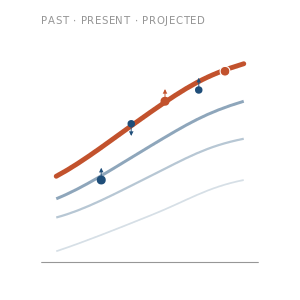
\includegraphics[height=6mm]{yc_logo.png}}
\end{frame}

% 2 ---------------------------------------------------------------------------
\begin{frame}{Motivation}
  \kicker{NII forecasting and IRRBB governance}
  \begin{itemize}
    \item Forecast accuracy for net interest income (NII) and interest-rate
          risk in the banking book (IRRBB) is central to earnings stability,
          balance-sheet management and supervisory credibility.
    \item Many institutions govern forecast performance with fixed deviation
          thresholds (3/4/5\%), even though forecast uncertainty widens with
          the horizon and the error process may be heavy-tailed. A flat limit
          therefore carries no consistent probabilistic interpretation.
    \item The paper develops an integrated, probability-coherent framework
          for monitoring NII forecast errors and assessing IRRBB limit
          breaches, calibrated to the bank's own empirical error
          distribution.
  \end{itemize}
\end{frame}

% 3 ---------------------------------------------------------------------------
\begin{frame}{Where forecast errors come from}
  \kicker{NII forecast construction}
  \begin{itemize}
    \item NII baselines are built under run-off, static or dynamic
          balance-sheet assumptions, combined with an interest-rate path
          (market forwards or house views) and pricing and behavioral
          inputs. Each assumption is a source of forecast error.
    \item The paper distinguishes sensitivities, responses of NII to
          prescribed shocks, from risk measures, statements about the
          probability distribution of outcomes. Escalation limits belong to
          the second category.
    \item The governance angle is distributional and horizon-aware: limits
          are calibrated to the empirical forecast-error distribution rather
          than attributing each miss causally.
  \end{itemize}
\end{frame}

% 4 ---------------------------------------------------------------------------
\begin{frame}{Horizon-specific, quantile-anchored thresholds}
  \kicker{The SEP fan-chart logic applied to escalation limits}
  \small Following the Federal Reserve's RMSE-based communication of forecast
  uncertainty, thresholds are anchored to the horizon-specific error scale:
  \[ c_{h,q} \;=\; z_q \cdot RMSE(h),
     \qquad z_{80}=0.84,\; z_{90}=1.28,\; z_{95}=1.64,\; z_{99}=2.33 \]
  under the Normal/RMSE mapping used for communication, with empirical
  quantiles replacing $z_q\,RMSE(h)$ where the error history warrants it.
  \begin{itemize}
    \item Escalation tiers then inherit a coverage interpretation: a
          $q$-tier limit is expected to be exceeded with probability $1-q$
          at every horizon, which no flat limit can deliver.
  \end{itemize}
\end{frame}

% 5 ---------------------------------------------------------------------------
\begin{frame}{A common unit across horizons}
  \kicker{Standardized exceedance score}
  \small Each realized relative error $e_{t,h}$ is expressed as a proportion
  of the 95\% boundary for its horizon,
  \[ S_{t,h} \;=\; \frac{\left|e_{t,h}\right|}{Q_h(0.95)}, \]
  so that dashboards report one number with the same meaning at every $h$.
  \begin{itemize}
    \item $S_{t,h}<1$ lies inside the 95\% band, $S_{t,h}\ge 1$ marks an
          exceedance, and the magnitude above one grades its severity.
    \item The score separates the monitoring object (a standardized
          statistic) from the governance object (the tier boundaries), so
          recalibration of limits does not change the reporting format.
  \end{itemize}
\end{frame}

% 6 ---------------------------------------------------------------------------
\begin{frame}{The outer tier: extreme value theory}
  \kicker{POT-GPD calibration of rare misses}
  \begin{itemize}
    \item Because NII forecast errors may be heavy-tailed, the outer
          escalation tier is calibrated by peaks-over-threshold: by the
          Pickands--Balkema--de Haan theorem, excesses over a high threshold
          converge to a Generalized Pareto Distribution.
    \item In the empirical illustration the EVT overlay is applied only to
          the outer tier, under the $\xi\to 0$ exponential-tail
          approximation with diagnostics, to stabilise deep tails estimated
          from few observations.
    \item The construction is analogous to Expected-Shortfall extensions of
          the Basel VaR traffic-light backtest: probabilistic coverage
          targets operationalised into governance tiers.
  \end{itemize}
\end{frame}

% 7 ---------------------------------------------------------------------------
\begin{frame}{Simulated thresholds by horizon}
  \kicker{N=120 per horizon · 5 exceedances at the 95\% threshold}
  \small Empirical thresholds of $|e_{t,h}|$ (relative NII forecasting
  errors) and the EVT outer tier:
  \begin{center}
  \begin{tabular}{lcccc}
    \toprule
    & $h=3$m & $h=6$m & $h=12$m & $h=24$m \\
    \midrule
    80\% & 0.99\% & 1.40\% & 1.96\% & 2.81\% \\
    90\% & 1.25\% & 1.74\% & 2.43\% & 3.46\% \\
    95\% & 2.01\% & 2.82\% & 4.00\% & 5.54\% \\
    EVT 97.5\% & 2.63\% & 3.73\% & 5.29\% & 7.36\% \\
    \bottomrule
  \end{tabular}
  \end{center}
  \vspace{1mm}
  Average exceedances $\hat\beta_h$ rise with the horizon as well: 1.21\%,
  1.79\%, 2.52\% and 3.55\%. Dispersion growth with $h$ is embedded in the
  limit definition itself.
\end{frame}

% 8 ---------------------------------------------------------------------------
\begin{frame}{Twelve limits versus one flat number}
  \kicker{Horizon-specific system vs flat 3/4/5\%}
  \begin{itemize}
    \item The 12-limit system (three tiers at four horizons) aligns
          exceedance rates across horizons: every tier means the same
          probability everywhere.
    \item Against flat 3/4/5\% limits the comparison shows fewer false
          alarms at long horizons, where flat limits over-penalise the
          naturally wider errors, and fewer missed tails at short horizons,
          where flat limits are too loose.
    \item Backtesting of the system is clean in the simulation, with
          threshold stability demonstrated across replications.
  \end{itemize}
\end{frame}

% 9 ---------------------------------------------------------------------------
\begin{frame}{Statistical validation}
  \kicker{Coverage, elicitability, decomposition}
  \begin{itemize}
    \item Interval-forecast evaluation follows Christoffersen (1998):
          unconditional coverage, whether the long-run frequency of
          exceedances matches the nominal level, and conditional coverage,
          whether exceedances are independent rather than clustered.
    \item Kupiec's proportion-of-failures test (1995) provides the simpler
          unconditional benchmark familiar from the 1996 Basel traffic-light
          framework for VaR backtesting.
    \item Quantile elicitability justifies the quantile as the reported
          functional, and a bias-dispersion decomposition separates
          structural misspecification from random variation in the error
          process.
  \end{itemize}
\end{frame}

% 10 --------------------------------------------------------------------------
\begin{frame}{The IRRBB extension}
  \kicker{Breach probabilities for $\Delta$NII limits}
  \begin{itemize}
    \item The methodology extends to IRRBB by quantifying the probability
          that limits on $\Delta$NII are breached solely due to forecast or
          model uncertainty, with no change in the underlying risk position.
    \item This maps model risk into risk-appetite language: a limit whose
          pure-noise breach probability is material is not measuring the
          intended exposure, which matters under the Basel IRRBB Standard
          (BCBS 368).
    \item Breach probabilities per horizon are directly suitable for ALCO
          reporting alongside the exceedance score.
  \end{itemize}
\end{frame}

% 11 --------------------------------------------------------------------------
\begin{frame}{Limitations and adoption path}
  \kicker{What the framework requires}
  \begin{itemize}
    \item Calibration is data-hungry at long horizons: the 24-month tier
          rests on few effective observations, which the EVT overlay
          mitigates but does not remove.
    \item Regime or model changes can break stationarity of the error
          process, requiring re-baselining and shadow backtests.
    \item At adoption the paper recommends wider bands or pooled-horizon
          estimation until the institution's own error history is long
          enough, with a sequenced implementation road map.
  \end{itemize}
\end{frame}

% 12 --------------------------------------------------------------------------
\begin{frame}{Implications}
  \kicker{For forecast governance}
  \begin{itemize}
    \item Escalation limits gain a coverage interpretation: management knows
          the probability content of every tier at every horizon, instead of
          a flat number that means a different probability at each $h$.
    \item Comparability across horizons is restored because dispersion
          growth is embedded in the limit definition, and
          conditional-coverage testing detects clustering of exceptions.
    \item The same architecture serves NII forecast monitoring and IRRBB
          limit design, giving one consistent statistical language for both.
  \end{itemize}
\end{frame}

% 13 --------------------------------------------------------------------------
\begin{frame}[plain]
  \vspace{12mm}
  {\fontsize{27}{31}\selectfont\bfseries\color{ycink}Thank you.\par}
  \vspace{6mm}
  {\normalsize\color{ycink}Marcin Dec\par}
  {\small\color{ycmuted}Kozminski University \& FAME|GRAPE, Warsaw\\
   mdec@kozminski.edu.pl · ORCID 0000-0002-6220-8267\par}
  \vspace{5mm}
  {\ttfamily\footnotesize\color{ycaccent}%
   Dec, M. When 3\% Means Nothing: Calibrating Escalation Limits to a\\
   Bank's Own Forecasting Error Distribution. SSRN 6276722.\\
   doi:10.2139/ssrn.6276722 · under peer review\par}
  \vfill
  \raisebox{-1mm}{
\includegraphics[height=6mm]{kozminski_logo.png}}\hspace{5mm}
  \raisebox{-1mm}{
\includegraphics[height=6mm]{grape_logo.png}}\hspace{5mm}
  \raisebox{-1mm}{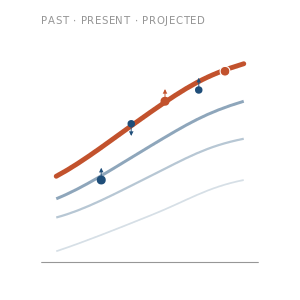
\includegraphics[height=6mm]{yc_logo.png}}
  \hfill{\ttfamily\scriptsize\color{ycmuted}yieldcartography.com/slides/escalation/}
\end{frame}

\end{document}
